\documentclass{beamer}

% --- Preamble: Theme and Packages ---

% Choose a theme for the presentation
\usetheme{Madrid}
\usecolortheme{default}

\usepackage{graphicx}   % To include images
\usepackage{booktabs}   % For professional tables
\usepackage{listings}   % For code snippets
\usepackage{xcolor}     % For custom colors in code

% Define Python style for code listings
\definecolor{codegreen}{rgb}{0,0.6,0}
\definecolor{codegray}{rgb}{0.5,0.5,0.5}
\definecolor{codepurple}{rgb}{0.58,0,0.82}
\definecolor{backcolour}{rgb}{0.95,0.95,0.92}

\lstdefinestyle{pythonstyle}{
    backgroundcolor=\color{backcolour},   
    commentstyle=\color{codegreen},
    keywordstyle=\color{magenta},
    stringstyle=\color{codepurple},
    basicstyle=\ttfamily\footnotesize,
    breakatwhitespace=false,         
    breaklines=true,                 
    captionpos=b,                    
    keepspaces=true,                 
    showspaces=false,                
    showstringspaces=false,
    showtabs=false,                  
    tabsize=2,
    language=Python
}
\lstset{style=pythonstyle}


% --- Presentation Information ---
\title[FloraDoc]{FloraDoc: AI-Powered Plant Disease Detection}
\author{Pratik Jadhav}
\institute{National Institute of Technology Calicut / Semester 1}
\date{\today}


% --- BEGIN DOCUMENT ---
\begin{document}

% --- Title Frame ---
\begin{frame}
    \titlepage
\end{frame}

% --- Table of Contents ---
\begin{frame}{Outline}
    \tableofcontents
\end{frame}

% --- SECTION 1: PROBLEM STATEMENT ---
\section{Problem Statement}
\begin{frame}{The Challenge: Agricultural Crop Loss}
    \begin{columns}
        \begin{column}{0.6\textwidth} % Left column for text
            \begin{block}{The Problem}
                Farmers and home gardeners often struggle with the early and accurate identification of plant diseases. This uncertainty leads to:
                \begin{itemize}
                    \item Significant crop loss and economic damage.
                    \item Incorrect application of pesticides, harming the environment.
                    \item Delays in treatment, allowing diseases to spread.
                \end{itemize}
            \end{block}
            \vspace{1cm}
            \begin{alertblock}{Our Goal}
                To develop a simple, accessible, and instant tool for diagnosing plant diseases using a smartphone.
            \end{alertblock}
        \end{column}
        \begin{column}{0.4\textwidth} % Right column for image
            \centering % Center the image within this column
            \begin{figure}
                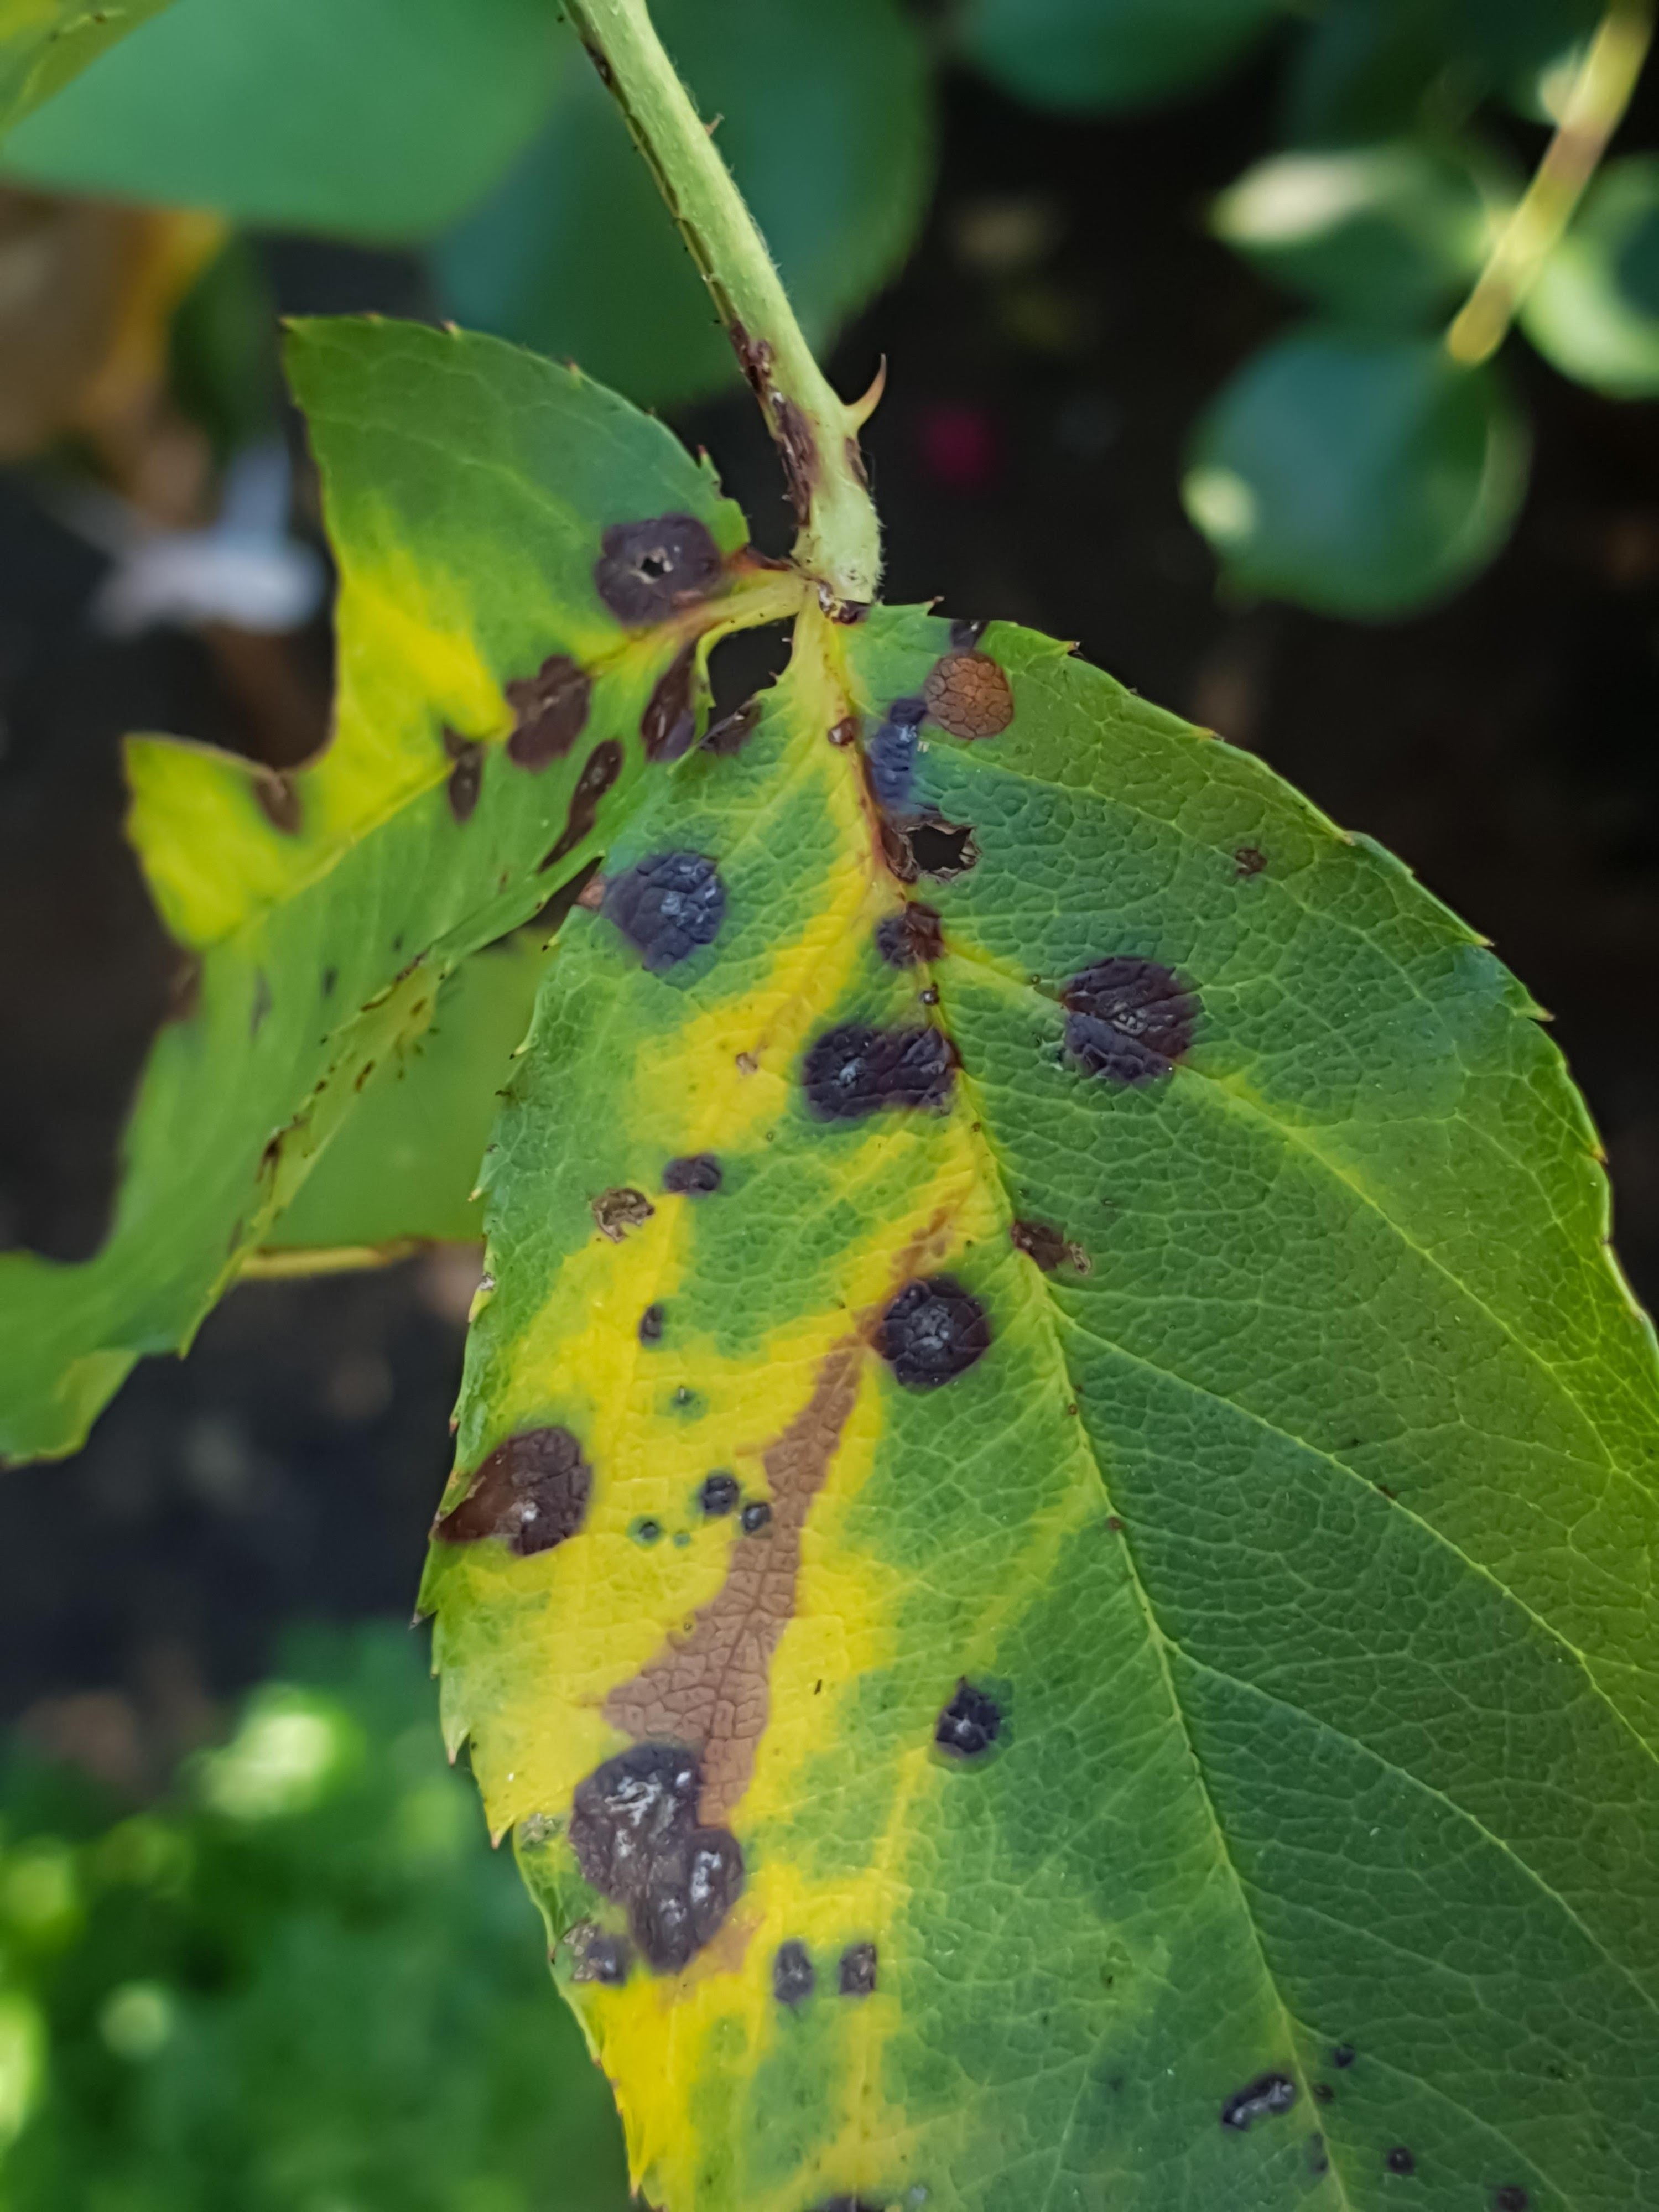
\includegraphics[width=\textwidth]{diseased_leaf.jpg}
                \caption{A leaf showing signs of disease.}
            \end{figure}
        \end{column}
    \end{columns}
\end{frame}

% --- SECTION 2: INTRODUCTION ---
\section{Introduction}
\begin{frame}{Introducing FloraDoc}
    \begin{center}
        \Large\textbf{Our Solution: A Mobile App for Instant Diagnosis}
    \end{center}
    
    \vspace{0.5cm}
    
    FloraDoc is a cross-platform mobile application that leverages the power of Artificial Intelligence to identify plant diseases from a single photograph.
    
    \begin{block}{Key Features}
        \begin{itemize}
            \item \textbf{Instant Identification:} Snap a photo of a plant leaf and get a diagnosis in seconds.
            \item \textbf{High Accuracy:} Powered by a deep learning model trained on thousands of images.
            \item \textbf{Treatment Suggestions:} Provides recommendations for organic and chemical treatments.
            \item \textbf{User-Friendly Interface:} Designed for simplicity and ease of use.
        \end{itemize}
    \end{block}
\end{frame}

% --- SECTION 3: DESIGN ---
\section{Design and Architecture}
\begin{frame}{System Architecture}
    \frametitle{How FloraDoc Works: A High-Level Overview}
    \begin{figure}
        \centering % Center the figure on the frame
        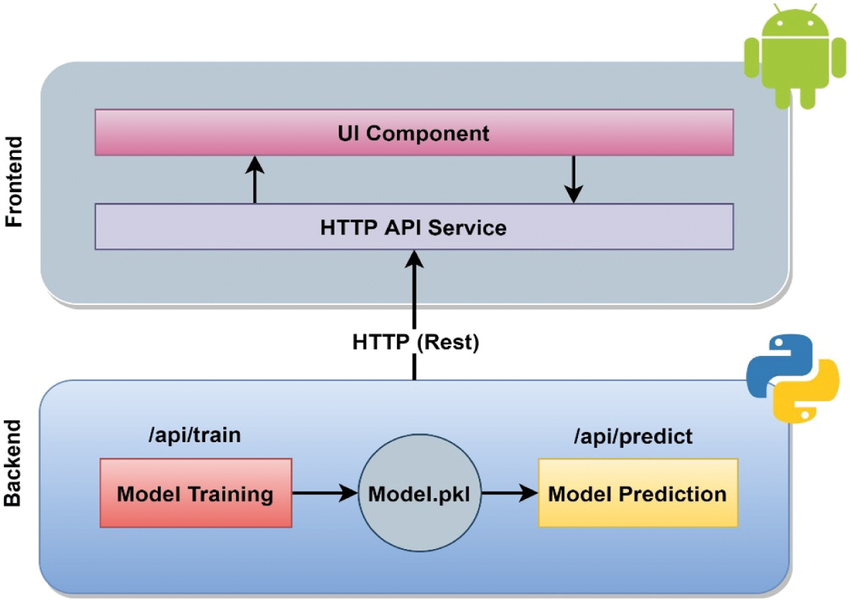
\includegraphics[width=0.8\linewidth]{architecture_diagram.png} % Adjusted width for better fit
        \caption{The three main components: Mobile App, Backend API, and ML Model.}
    \end{figure}
    
    \begin{itemize}
        \item \textbf{Mobile Client (Frontend):} The user interface for capturing images and displaying results.
        \item \textbf{Backend Server (API):} Manages user requests, processes images, and communicates with the machine learning model.
        \item \textbf{ML Model:} A Convolutional Neural Network (CNN) that performs the image classification.
    \end{itemize}
\end{frame}

% --- SECTION 4: IMPLEMENTATION ---
\section{Implementation Details}
\begin{frame}{Technology Stack}
    \frametitle{The Tools and Technologies We Used}
    \begin{columns}
        % Column 1: Frontend & Backend
        \begin{column}{0.5\textwidth}
            \begin{block}{Frontend (Mobile App)}
                \begin{itemize}
                    \item \textbf{Framework:} Flutter
                    \item \textbf{Language:} Dart
                    \item \textbf{Key Libraries:} \texttt{camera}, \texttt{http}
                \end{itemize}
            \end{block}
            
            \begin{block}{Backend (API Server)}
                \begin{itemize}
                    \item \textbf{Framework:} FastAPI
                    \item \textbf{Language:} Python
                    \item \textbf{Deployment:} Docker, AWS
                \end{itemize}
            \end{block}
        \end{column}
        
        % Column 2: ML Model
        \begin{column}{0.5\textwidth}
            \begin{block}{Machine Learning Model}
                \begin{itemize}
                    \item \textbf{Framework:} TensorFlow/Keras
                    \item \textbf{Architecture:} MobileNetV2 (CNN)
                    \item \textbf{Dataset:} PlantVillage Dataset
                    \item \textbf{Training:} Transfer Learning
                \end{itemize}
            \end{block}
        \end{column}
    \end{columns}
\end{frame}

\begin{frame}[fragile]{Implementation Snippet: Backend API}
    \frametitle{A Look at the Prediction Endpoint}
    
    Here is a simplified version of the Python code (using FastAPI) that handles image uploads and returns a prediction.
    
    \begin{lstlisting}[language=Python, caption={FastAPI Prediction Endpoint}]
from fastapi import FastAPI, UploadFile, File
from PIL import Image
import tensorflow as tf

app = FastAPI()
model = tf.keras.models.load_model("plant_disease_model.h5")
class_names = ["Healthy", "Rust", "Powdery Mildew"]

@app.post("/predict")
async def predict(file: UploadFile = File(...)):
    # Read and preprocess the image
    image = Image.open(file.file)
    image = image.resize((224, 224))
    img_array = tf.keras.utils.img_to_array(image)
    img_array = tf.expand_dims(img_array, 0) # Create batch

    # Make prediction
    predictions = model.predict(img_array)
    score = tf.nn.softmax(predictions[0])
    
    # Return result
    return {
        "disease": class_names[tf.argmax(score)],
        "confidence": f"{100 * tf.reduce_max(score):.2f}%"
    }
    \end{lstlisting}
\end{frame}


% --- FINAL SLIDE ---
\begin{frame}{Conclusion \& Questions}
    \begin{center}
        \Huge\bfseries Thank You!
        \vspace{1cm}
        
        \Large Questions?
    \end{center}
\end{frame}

\end{document}